\documentclass{article}
\usepackage{xcolor}
\usepackage{tikz}
\usetikzlibrary{arrows.meta,positioning,shapes.geometric}
\usepackage[margin=0pt,paperwidth=28cm,paperheight=30cm]{geometry}
\pagestyle{empty}
\parindent=0pt

\begin{document}
\vspace*{6pt}\hspace*{6pt}
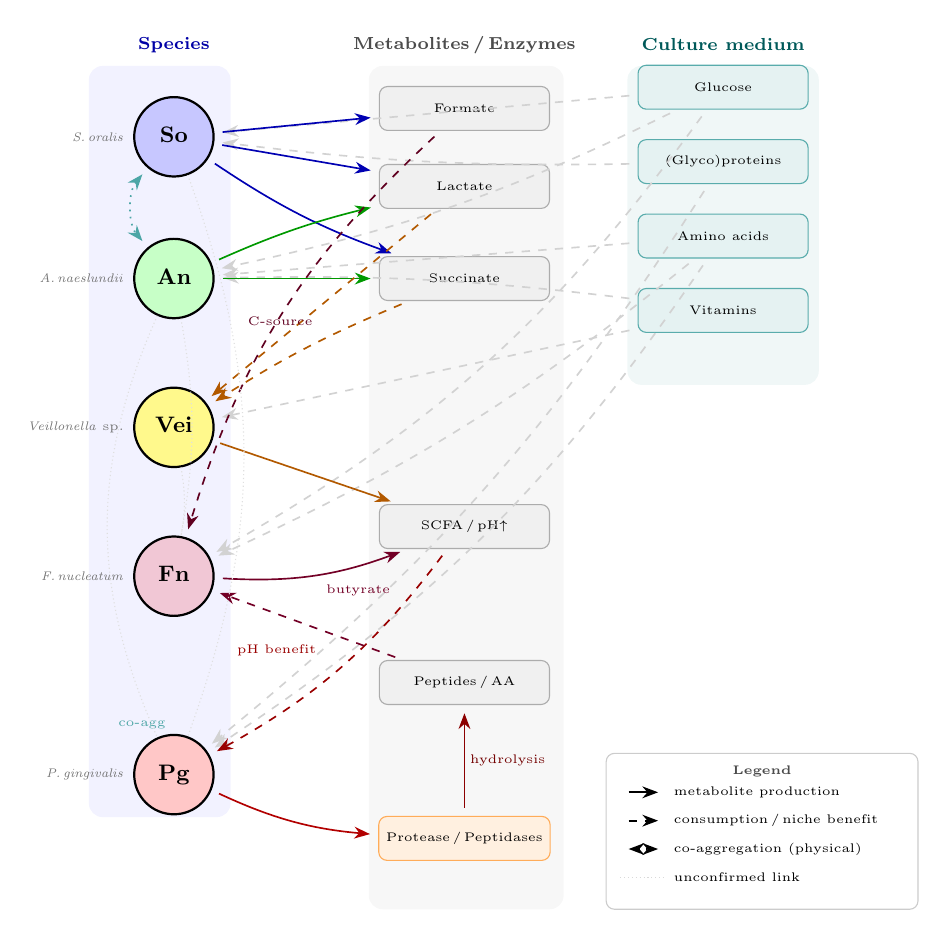
\begin{tikzpicture}[scale=0.90, every node/.style={transform shape},
    sp/.style={circle, draw, thick, minimum size=1.12cm,
               font=\small\bfseries, inner sep=0pt},
    met/.style={rounded corners=3pt, draw=gray!65, font=\tiny,
                fill=gray!12, inner sep=3pt,
                minimum width=2.4cm, minimum height=0.62cm, align=center},
    enz/.style={rounded corners=3pt, draw=orange!65, font=\tiny,
                fill=orange!12, inner sep=3pt,
                minimum width=2.4cm, minimum height=0.62cm, align=center},
    med/.style={rounded corners=3pt, draw=teal!65, font=\tiny,
                fill=teal!10, inner sep=3pt,
                minimum width=2.4cm, minimum height=0.62cm, align=center},
    prd/.style={->, >=Stealth, semithick, shorten <=3pt, shorten >=3pt},
    cns/.style={->, >=Stealth, semithick, dashed,  shorten <=3pt, shorten >=3pt},
    phy/.style={<->, >=Stealth, semithick, dotted, shorten <=3pt, shorten >=3pt},
    lbl/.style={font=\tiny, inner sep=0pt},
]

% ─── column backgrounds ────────────────────────────────────────────────────
\fill[blue!5,  rounded corners=5pt] (-1.2, -1.3) rectangle (0.8, 9.3);
\fill[gray!6,  rounded corners=5pt] (2.75, -2.6) rectangle (5.5, 9.3);
\fill[teal!6,  rounded corners=5pt] (6.4,  4.8)  rectangle (9.1, 9.3);

% ─── column headers ────────────────────────────────────────────────────────
\node[font=\scriptsize\bfseries, text=blue!65!black]  at (0,    9.6) {Species};
\node[font=\scriptsize\bfseries, text=gray!60!black]  at (4.1,  9.6) {Metabolites\,/\,Enzymes};
\node[font=\scriptsize\bfseries, text=teal!70!black]  at (7.75, 9.6) {Culture medium};

% ─── culture medium nodes ──────────────────────────────────────────────────
\node[med] (mGlu) at (7.75, 9.0)  {Glucose};
\node[med] (mPro) at (7.75, 7.95) {(Glyco)proteins};
\node[med] (mAA)  at (7.75, 6.9)  {Amino acids};
\node[med] (mVit) at (7.75, 5.85) {Vitamins};

% ─── metabolite / enzyme nodes (x=4.1) ────────────────────────────────────
\node[met] (For)  at (4.1,  8.7)  {Formate};
\node[met] (Lac)  at (4.1,  7.6)  {Lactate};
\node[met] (Suc)  at (4.1,  6.3)  {Succinate};
\node[met] (SCFA) at (4.1,  2.8)  {SCFA\,/\,pH$\uparrow$};
\node[met] (Pep)  at (4.1,  0.6)  {Peptides\,/\,AA};
\node[enz] (Enz)  at (4.1, -1.6)  {Protease\,/\,Peptidases};

% ─── species nodes (x=0) ──────────────────────────────────────────────────
\node[sp, fill=blue!22]   (So)  at (0,  8.3)  {\strut So};
\node[sp, fill=green!22]  (An)  at (0,  6.3)  {\strut An};
\node[sp, fill=yellow!45] (Vei) at (0,  4.2)  {\strut Vei};
\node[sp, fill=purple!22] (Fn)  at (0,  2.1)  {\strut Fn};
\node[sp, fill=red!22]    (Pg)  at (0, -0.7)  {\strut Pg};

% ─── species full names ────────────────────────────────────────────────────
\node[lbl, anchor=east, text=black!55] at (-0.7,  8.3)  {\textit{S.\,oralis}};
\node[lbl, anchor=east, text=black!55] at (-0.7,  6.3)  {\textit{A.\,naeslundii}};
\node[lbl, anchor=east, text=black!55] at (-0.7,  4.2)  {\textit{Veillonella} sp.};
\node[lbl, anchor=east, text=black!55] at (-0.7,  2.1)  {\textit{F.\,nucleatum}};
\node[lbl, anchor=east, text=black!55] at (-0.7, -0.7)  {\textit{P.\,gingivalis}};

% ─── physical co-aggregation ──────────────────────────────────────────────
\draw[phy, blue!50!green!70]
    (So) to[bend right=40] (An)
    node[midway, left=3pt, lbl, text=blue!50!green!70] {co-agg};

% ─── medium → species ─────────────────────────────────────────────────────
\draw[cns, gray!35] (mGlu) -- (So);
\draw[cns, gray!35] (mGlu) to[bend left=7]  (An);
\draw[cns, gray!35] (mGlu) to[bend left=12] (Fn);
\draw[cns, gray!35] (mPro) to[bend left=4]  (So);
\draw[cns, gray!35] (mPro) to[bend left=9]  (Pg);
\draw[cns, gray!35] (mAA)  -- (An);
\draw[cns, gray!35] (mAA)  to[bend left=7]  (Fn);
\draw[cns, gray!35] (mAA)  to[bend left=11] (Pg);
\draw[cns, gray!35] (mVit) to[bend right=4] (An);
\draw[cns, gray!35] (mVit) -- (Vei);

% ─── So → Formate, Lactate, Succinate ─────────────────────────────────────
\draw[prd, blue!70!black] (So) -- (For);
\draw[prd, blue!70!black] (So) -- (Lac);
\draw[prd, blue!70!black] (So) to[bend right=7] (Suc);

% ─── An → Lactate, Succinate ──────────────────────────────────────────────
\draw[prd, green!60!black] (An) to[bend left=5] (Lac);
\draw[prd, green!60!black] (An) -- (Suc);

% ─── Lactate, Succinate → Vei ─────────────────────────────────────────────
\draw[cns, orange!70!black] (Lac) -- (Vei);
\draw[cns, orange!70!black] (Suc) to[bend right=5] (Vei);

% ─── Vei → SCFA ───────────────────────────────────────────────────────────
\draw[prd, orange!70!black] (Vei) -- (SCFA);

% ─── Fn → SCFA (butyrate) ─────────────────────────────────────────────────
\draw[prd, purple!60!black] (Fn) to[bend right=12] (SCFA);
\node[lbl, text=purple!60!black] at (2.6, 1.9) {butyrate};

% ─── SCFA / pH↑ → Pg ──────────────────────────────────────────────────────
\draw[cns, red!60!black] (SCFA) to[bend left=12] (Pg);
\node[lbl, text=red!60!black] at (1.45, 1.05) {pH benefit};

% ─── Pg → Enz → Pep → Fn ─────────────────────────────────────────────────
\draw[prd, red!70!black]    (Pg)  to[bend right=10] (Enz);
\draw[prd, red!55!black]    (Enz) -- (Pep)
    node[midway, right=2pt, lbl, text=red!45!black] {hydrolysis};
\draw[cns, purple!60!black] (Pep) -- (Fn);

% ─── Formate → Fn (confirmed C-source) ───────────────────────────────────
\draw[cns, purple!50!black] (For) to[bend right=15] (Fn);
\node[lbl, text=purple!50!black] at (1.5, 5.7) {C-source};

% ─── unconfirmed species pairs ────────────────────────────────────────────
\draw[gray!25, densely dotted] (So)  to[bend left=20]  (Pg);
\draw[gray!25, densely dotted] (An)  to[bend right=24] (Pg);
\draw[gray!25, densely dotted] (Vei) to[bend left=10]  (Fn);
\draw[gray!25, densely dotted] (An)  to[bend left=10]  (Fn);

% ─── legend (lower right, below teal box) ─────────────────────────────────
\fill[white, rounded corners=3pt] (6.1, -2.6) rectangle (10.5, -0.4);
\draw[gray!40, rounded corners=3pt, thin] (6.1, -2.6) rectangle (10.5, -0.4);
\node[font=\tiny\bfseries, text=black!70] at (8.3, -0.65) {Legend};
\draw[prd, black]              (6.3, -0.95) -- (6.95, -0.95);
\node[lbl, anchor=west] at (7.05, -0.95) {metabolite production};
\draw[cns, black]              (6.3, -1.35) -- (6.95, -1.35);
\node[lbl, anchor=west] at (7.05, -1.35) {consumption\,/\,niche benefit};
\draw[phy, black]              (6.3, -1.75) -- (6.95, -1.75);
\node[lbl, anchor=west] at (7.05, -1.75) {co-aggregation (physical)};
\draw[gray!30, densely dotted] (6.3, -2.15) -- (6.95, -2.15);
\node[lbl, anchor=west] at (7.05, -2.15) {unconfirmed link};

\end{tikzpicture}
\end{document}
